\section{Introduction} \label{sec:introduction}

The rising popularity of statically typed functional languages led to
the concept of ``type-driven development'' (hereinafter referred to as TDD).
Typed holes let us write a program top-down and leave the parts we do not know
how to write incomplete. The parts we have already written dictate what the
types of remaining parts should be, and those types guide us when we try to
figure out how we should fill the incomplete parts.
In other words, in TDD we can write our programs incrementally. This not only
lets us type check our program at every step, it also gives us clever
hints about the future steps, based on the types and the local context.
Especially as dependent types gradually sneak in to mainstream languages, like
they already have to Haskell\cite{eisenberg} and Scala\cite{scalaDep} now, we
predict that TDD will only get more popular.

Interactive editing based on types has been used in proof assistants for a long
time; the LCF system\cite{lcf} and its successors HOL and
Isabelle\cite{isabelle} allow users to prove theorems
incrementally. Users type in commands that update the proof state by
changing the goal, or by creating subgoals. These commands are called
tactics and even though they also generate a proof term in the style
of Curry-Howard isomorphism at the end, they only allow the user to change the
proof term indirectly.
Inspired by these systems, there were also proof assistants that let users
change the proof term directly by incrementally building it
up\footnote{Changing the proof term indirectly with tactics is also called
backward reasoning, and incrementally building up the proof term is called
forward reasoning.}. One of the earliest such proof assistants was the ALF proof
editor\cite{ALF}, and the idea was developed further by Epigram\cite{epigram}
and Agda\cite{agda}.  The recent popularity of TDD in more mainstream
functional programming is built upon the legacy of these interactive proof
assistants.

On the practical programming side, the traditional programming
workflow that depends on saving a file and trying to compile (or run) with
every edit has changed with the advancement of integrated development environments (IDEs),
programs that have certain functionalities such as code completion, syntax
checking, displaying compiler error messages on corresponding lines, displaying
documentation etc. These features are convenient, but they are different from
TDD. While IDEs can also use types to assist the user, they do not direct the
entire development process around types per se. TDD is not a program, it is
merely a style of programming in which the development process takes the form
of a conversation between the type-checker/compiler and the user's editor/IDE.
However, this requires certain changes to the compiler, such as being able to
type-check incomplete expressions and definitions.\cite{tdd}

The kind of change that is important for this work is the editor
interaction mode (or the IDE mode, as it is called in Idris\cite{idris}) that
lets the editor talk to the compiler\footnote{To avoid any confusion,
we should mention that there are two different parts of an editor interaction
mode. The first is a plugin to the editor, often written in the script language
of the editor, such as Emacs Lisp or VimL. The second part is a separate
program that does the heavy lifting of the editing features that work with the
language itself.  \path{ghc-mod} in Haskell and \path{agda-mode} in Agda would
be perfect examples for the second part. We will call these parts the frontend
and backend of the editor interaction mode, respectively.  When we talk about
the language the editor interaction mode is implemented, we mean the language
used in the backend, because the language used in the frontend depends on the
editor.}.
There are various existing examples of compilers and editors
that do this sort of interaction:
Proof General\cite{pg} and CoqIDE for Coq\cite{coq},
the Emacs mode\cite{agdamode} for Agda,
the Emacs mode\cite{idrismode} for Idris,
jEdit\cite{isabellejedit} for Isabelle,
and recently the editor mode of Lean\cite{lean}.
Among these examples, Idris is the only language that prioritizes general
purpose programming rather than theorem proving\cite{idrisfaq}, but that does
not mean TDD is of less importance for Idris. On the contrary, this should
be the first step of convincing programmers to adopt TDD, since
editor interaction provides decent tools to help them write programs faster.

Before we proceed to describe this work,
it is imperative to understand what an editor action exactly is.
Editor actions are commands in the editor that make a meaningful
change in your code, or one that gives you some information about your
code. For example, if you are trying to define a function to compute the height
of a binary tree\footnote{The \texttt{\IdrisKeyword{\%name}} directive here tells
Idris how to generate new names for trees. This is not necessary.}, you can
just start by writing the type for the function.

\vspace{1em}
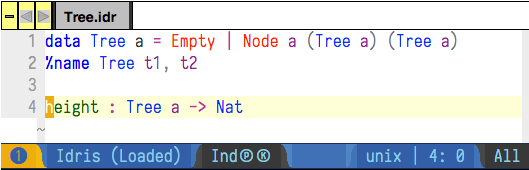
\includegraphics[scale=0.6]{edit1}

Note that initially we only declared the type of the function, and nothing
else. To get an initial incomplete definition, we can run the editor action
``Add initial match clause to type declaration'', while the cursor is on the
type declaration.

\vspace{1em}
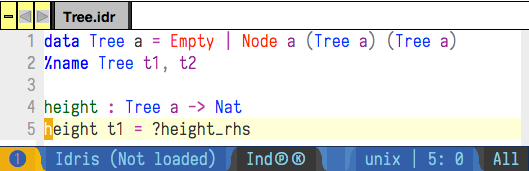
\includegraphics[scale=0.6]{edit2}

Now we have a definition for \fn{height} that takes one argument \bn{t1}, and
returns \hole{height_rhs}. This is clearly incomplete; we want to change
the return value based on what \bn{t1} is. So the next step would be to inspect
what values \bn{t1} can take. We can put the cursor on \bn{t1} and then run the
editor action ``Case split pattern variable''.

\vspace{1em}
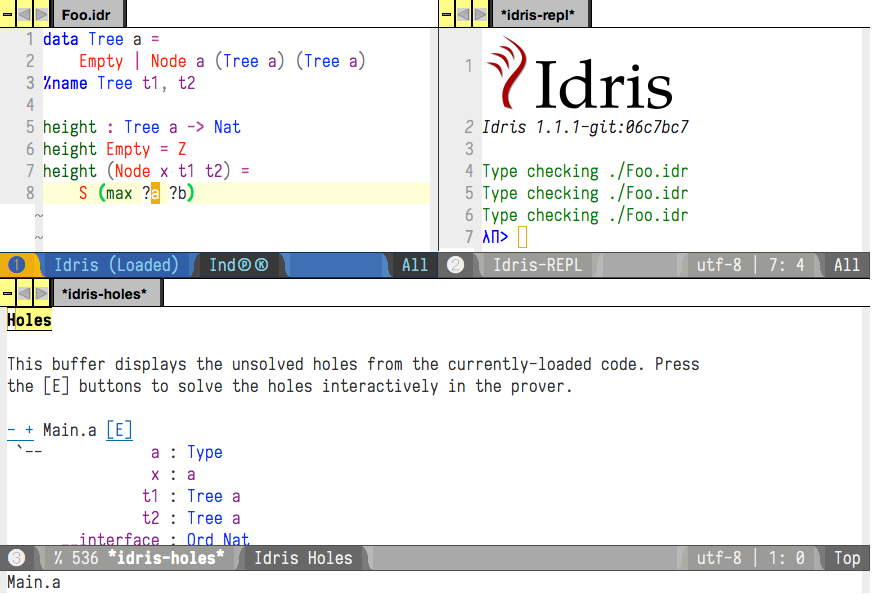
\includegraphics[scale=0.6]{edit3}

Now we have two holes that we have to complete, namely \hole{height_rhs1} and
\hole{height_rhs2}. When the cursor is on one of the holes, we can run the
editor action ``Display type'' and see what type of expression should replace
the hole, and what names are in the local context, i.e. are available to use
when writing that expression.

\vspace{1em}
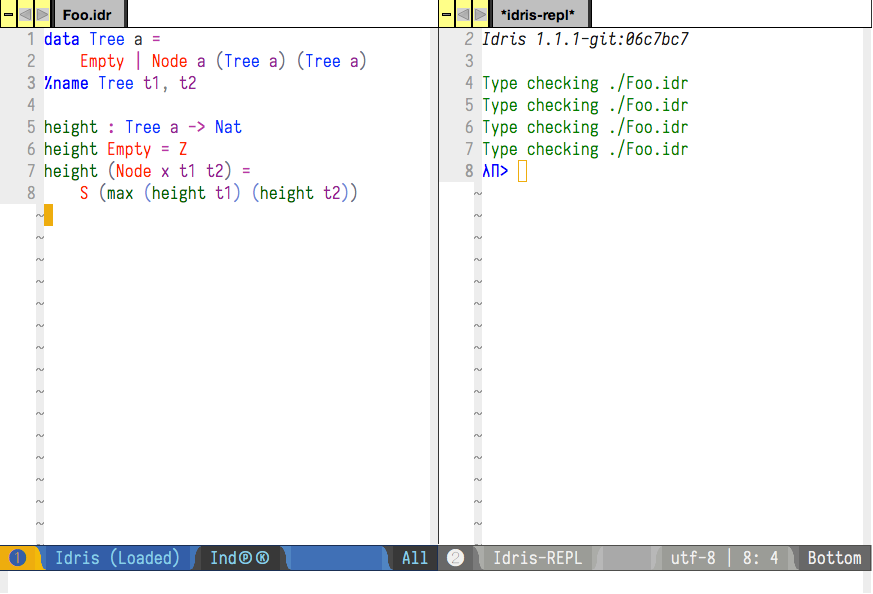
\includegraphics[scale=0.6]{edit4}

Finishing this function from here is trivial, so we will not proceed further.
However, this example shows how much editor actions can shape your
overall programming experience.

Now that we are familiar with what an editor action is, we can describe what
this project is about. The editor actions we reviewed above are features embedded
in the compiler. If you want to define a new action, the only way possible is
to change the compiler source code and build your own version of the compiler,
and then edit the source code of your editor mode to use that feature you
added. This is clearly far from ideal; no one should have to fork a compiler
just to add a custom editor action. Maintaining a compiler fork and
navigating through the compiler source code are usually not in the skill sets
of most users.

Therefore we want to provide users a way to write custom editor actions. Our
solution for this is to make use of elaborator reflection\cite{elabref} in
Idris, which is a metaprogramming machinery that allows users to automate the
construction of proofs and programs, by reflecting the elaborator
monad\cite{idris} in the Idris compiler. Christiansen and Brady showed that
this mechanism is powerful enough to replace the old tactic
language\cite{elabref} that existed in the previous versions of Idris, which is
now deprecated in favor of elaborator reflection.

Elaborator reflection adds a primitive monad \Elab\ to Idris itself, in which
type-checking and normalizing terms, looking up types and definitions of
functions are monadic actions\footnote{These monadic actions are still called
tactics, especially if they change the goal queue or the local context, hence the
title of this thesis. Note that whenever we use the word ``tactic'' in the
context of Idris, we exclusively refer to the monadic \Elab\ actions, not the
old tactic language.}.
This thesis argues that these actions provide a nice interface with which users
can define their custom editor actions. This has the following advantages:

\begin{itemize}
\item Implementations of the Idris editor actions mentioned above are
built-into the compiler and they are written in Haskell. This work will allow
us to rewrite them in Idris as \Elab\ actions. This way we can remove these
parts from the compiler and move them into an Idris library.
\item Abilities of the editor interaction mode is extended from the
current built-in features to anything that can be done with tactics.
\item Defining editor actions with a monadic interface allows us to
compose them easily. For instance, if we had case splitting as an \Elab\
action, we could define a tactic to case split on many arguments at the same time.
\end{itemize}

The ability to run tactics as editor actions has a consequence
that we have not explored much in this thesis.
Idris programs are usually meant to be executed, unlike Coq or
Agda programs, which are usually only meant to be type checked.\footnote{Of
  course there are backends for these languages, such as the OCaml
  backend for Coq and the Haskell backend for Agda.}
This means Idris programs will be compiled more often than Agda or Coq in the long run,
since not much code is added to proofs after its completion, but practical programs tend to change in time. Therefore, minimizing compile time is more of a priority for Idris.
Idris tactics generate proof terms in compile time, but the
compilation can take a long time for complex tactics\footnote{Similar problems
are observed in Coq. For example, theorems that use the famous \path{omega}
tactic that decides Presburger arithmetic take a long time to compile, and it
usually generates a huge proof term.},
not to mention that the implementation of elaborator
reflection in Idris has significant performance issues.\cite{leanmeta}
Yet we still want to utilize complex tactics to generate proofs or terms.
Using edit-time tactics, one would run a tactic once from the editor, generate
the proof term and serialize and send that to the editor and put it back in the
file.
If we think of the differences between the traditions of writing the proof
terms directly and writing tactics, the former more common in Agda and Idris
and the latter in Coq and Isabelle, this work will constitute a one way bridge
between the two, by making use of the elaborator reflection to create proof
terms in the editor in a smarter and quicker way.

The problem with that approach is that the generated proof terms can be (and
often are) gigantic and hideous, especially if generating a minimal proof term
is not a priority for the tactic we are using.
If there was a generic mechanism to simplify and minimize the generated proof
terms, and even write them in a way that makes use of dependent pattern
matching, then this could have been a more usable consequence of this work.
Ideally, we would want the artifact we are handing in to the reader of our
proofs to look just like what it would be if we had not used this system.
We leave that for future work.  However, even without proof simplification,
this still could be a last resort solution to repeated long compile times for
tactics.

To achieve the advantages listed above, we make the following specific contributions:
\vspace{-1em}
\begin{itemize}
\item We extend the primitive \Elab\ monad with the necessary primitive monadic
actions that make writing an editor action with elaborator reflection possible.
\item We define an Idris interface (or type class in Haskell terminology)
called \ty{Editorable} for serializing and deserializing Idris expressions.
For the reflected type that represents the core language terms of Idris,
implementations of this interface are primitives.
\item We add an interval map in which keys are intervals of source code
  positions (pair of line and column numbers) and values are local contexts at
    those positions. This allows us to inspect what variables are available to
    use even when we are not on a hole.
\item The current proof search mechanism in Idris is not particularly advanced.
We write an alternative proof search tactic called Hezarfen, a full-blown
theorem prover for intuitionistic propositional logic, and then we show how
to use this on holes when we are in the editor.
% Details can be found in \autoref{ssec:hezarfen}.
\item We define a case-split tactic that can be run from the editor, which can
replace the hard-coded case-split editor action.
\end{itemize}

In \autoref{sec:background}, we will go over the basics of the Idris
programming language and its metaprogramming mechanics.

Now that we have an idea about the motivations for such a feature, we will
discuss its design in \autoref{sec:design} and its implementation in
\autoref{sec:implementation}.


% One way to do this would be to have compiler plugins, like
% GHC\footnote{Users can write compiler GHC plugins in Haskell starting from GHC 7.2.1.
% \url{https://downloads.haskell.org/~ghc/7.2.1/docs/html/users_guide/compiler-plugins.html}}
% and Coq\footnote{Users can write compiler Coq plugins in OCaml.}
% However, the Idris compiler does not have a plugin system, and writing one for
% this purpose would be an overkill.



% Let's imagine a use case for such a feature.
% \begin{Verbatim}[framesep=2mm, label=\footnotesize{\normalfont{Idris}}, labelposition=topline]
% \fn{swap3} : \ty{(}\IdrisImplicit{a}\ty{,} \IdrisImplicit{b}\ty{,} \IdrisImplicit{c}\IdrisType{)} -> \ty{(}\IdrisImplicit{c}\ty{,} \IdrisImplicit{b}\IdrisType{,} \IdrisImplicit{a}\ty{)}
% \fn{swap3} \bn{x} = \IdrisMetavar{?\IdrisMetavar{p}}
% \end{Verbatim}
% We have a 3-tuple\footnote{n-tuples are nested right-associative pairs in
% Idris.} as an argument, and we need to access every element in that tuple.
% If we case split on the argument \path{x}, that pattern will turn into
% a pair. However we need the full \path{(a, b, c)} pattern in this
% case. We can case split again on the second component of the pair and get the
% 3-tuple pattern.
% For one function this repetition might not seem like a big deal, but if we need
% to do this numerously, we might want a way to automate that with a
% tactic.\footnote{Similar to the \path{unproduct} tactic in the Pruviloj library
% for Idris, but for case splitting.}

% Case splitting on a nested tuple might seem like a mindless task. What if we
% had a data type that required us to be clever when we are case splitting,
% then doing that for every function would get exhausting.
% Red-black trees\cite{okasakiRedBlack} are a good example of that.
% Suppose we want to balance a red-black tree, and we want to rotate the tree in
% the cases where we have two red nodes consecutively. We want to write some
% functions to rotate within the left and right subtrees. If we make use of
% dependent types to ensure certain properties about our tree, then pattern
% matching on our trees will be difficult to write by hand. However, we could
% write a tactic that does that for us. Moreover, the interesting cases are when
% we have two consecutive red nodes, so we might want to list them first in our
% patterns.  An Agda formalization of the tree rotation was previously given by
% Licata\cite{licataOPLSS}. In \autoref{ssec:rbt}, we first describe an Idris
% equivalent of that code, and then define a tactic to generate cases for
% rotation.
